\section{Marco teórico}

\begin{frame}{El problema: Medir la geometría de los poros}
    \begin{columns}[T]
        \column{0.5\textwidth}

        \begin{block}{Material: AAO}
            Membrana nanoestructurada con poros cilíndricos organizados en red hexagonal. Sus propiedades ópticas y mecánicas dependen de la geometría de los poros.
        \end{block}

        \column{0.5\textwidth}

        \begin{center}
            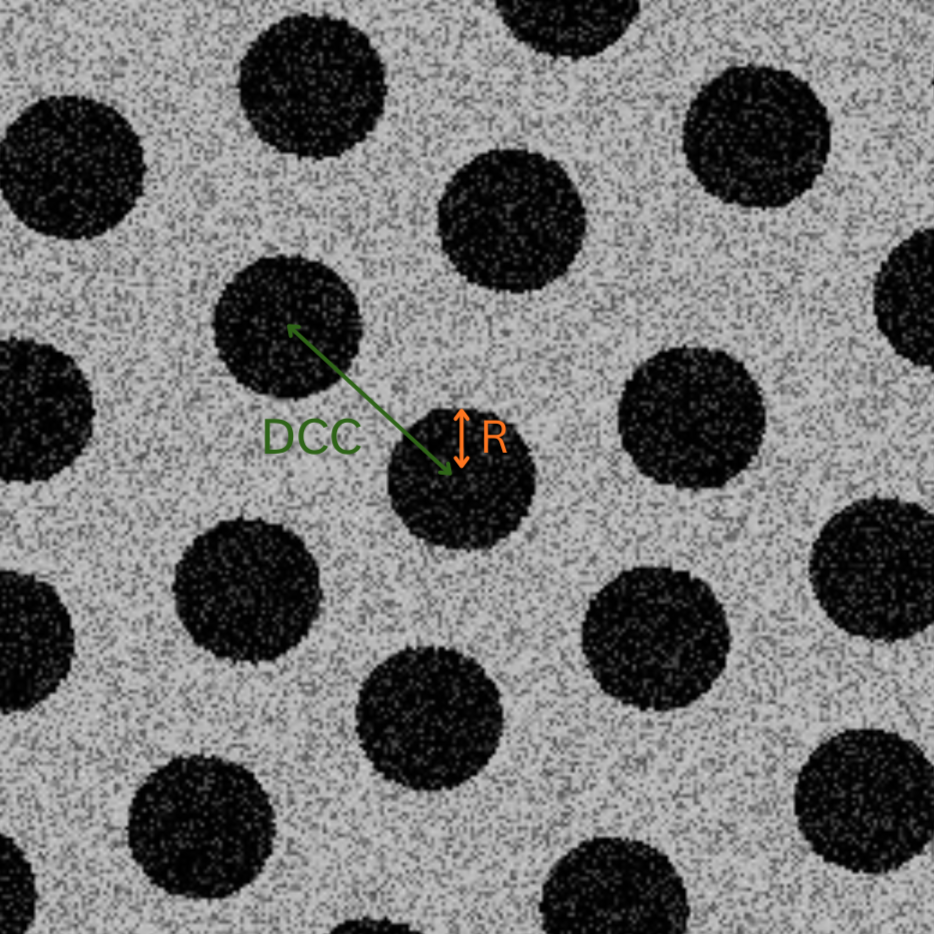
\includegraphics[width=0.7\textwidth]{chapters/introduction/ImagenAAO.png}
        \end{center}

    \end{columns}
\end{frame}